\documentclass[border=2mm]{standalone}
\usepackage{pgfplots}
\pgfplotsset{compat=1.18}
\usetikzlibrary{arrows.meta, 
  calc, 
  positioning, 
  decorations.pathreplacing, 
  calligraphy}

\usepackage{xcolor}
\definecolor{den-1}{HTML}{111111}   % Đen #111111
\definecolor{den-2}{HTML}{222222}   % Đen #222222
\definecolor{den-3}{HTML}{333333}   % Đen #333333
\definecolor{den-4}{HTML}{444444}   % Đen #444444
\definecolor{den-5}{HTML}{555555}   % Đen #555555
\definecolor{den-6}{HTML}{666666}   % Đen #666666

\definecolor{do-1}{HTML}{440000}   % Đỏ #440000 trầm hơn, hợp với đen #111111
\definecolor{do-2}{HTML}{660000}   % Đỏ #660000 sẫm, hợp với đen #222222
\definecolor{do-3}{HTML}{880000}   % Đỏ #880000 đậm vừa, hợp với đen #333333
\definecolor{do-4}{HTML}{AA0000}   % Đỏ #AA0000 tươi vừa, hợp với đen #444444
\definecolor{do-5}{HTML}{CC0000}   % Đỏ #CC0000 tươi hơn, hợp với đen #555555
\definecolor{do-6}{HTML}{EE0000}   % Đỏ #EE0000 sáng hơn, hợp với đen #666666

% Thiết lập vị trí đặt nhãn gốc tọa độ
\tikzset{
  >=Stealth,
  originlabel/.style={
    font=\small\sf,
    anchor=north east, % Vị trí tương đối so với gốc
    yshift=-0.1ex,     % Điều chỉnh vị trí dọc một chút
    xshift=-0.1ex      % Điều chỉnh vị trí ngang một chút
  }
}


\begin{document}

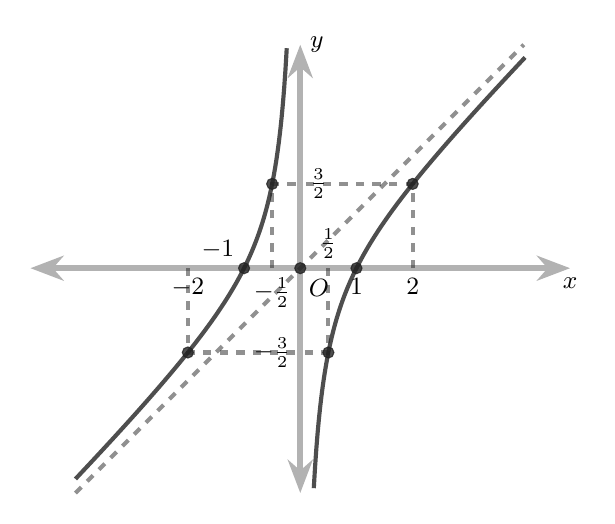
\begin{tikzpicture}
  \begin{axis}[
    font=\small\sf,
    axis lines = middle,
    axis line style={<->, line width=2pt, color=den-6!50},
    xlabel=$x$, ylabel=$y$,
    xlabel style={below, font=\small\sf},
    ylabel style={right, font=\small\sf},
    % ymin=-5.65, ymax=7.65,
    % ymin=-5.65, ymax=7.65,
    % width=12cm, height=8cm,
    xtick={},
    xticklabels={},
    xtick style={draw=none},
    ytick={1},    
    yticklabels={}, 
    ytick style={draw=none},  
    tick label style={font=\footnotesize\sf},
    clip=false,
    axis equal,
  ]

    \node[originlabel] at (axis cs:.0,0) [below right] {$O$};
    \node at (axis cs:1,0) [below] {$1$};
    \node at (axis cs:1/2,0) [above] {$\frac{1}{2}$};
    \node at (axis cs:-1/2,0) [below] {$-\frac{1}{2}$};
    \node at (axis cs:-1,0) [above left] {$-1$};
    % \node at (axis cs:0,-1) [below left] {$-1$};
    \node at (axis cs:2,0) [below] {$2$};
    \node at (axis cs:-2,0) [below] {$-2$};
    \node at (axis cs:0,3/2) [right] {$\frac{3}{2}$};
    \node at (axis cs:0,-3/2) [left] {$-\frac{3}{2}$};

    \addplot[domain=-4:4,
    restrict y to domain=-4:4, 
    samples=350, line width=1.5pt, color=den-2, opacity=.8] 
        {x-1/x};
    \addplot[dashed, domain=-4:4,
    restrict y to domain=-4:4, 
    samples=350, line width=1.5pt, color=den-2, opacity=.5] 
        {x};
    \addplot[only marks, mark size=2pt, mark=*, color=den-2, opacity=.8] coordinates {
        (1,0)
        (-1,0)
        (0,0)
        (2,3/2)
        (-2,-3/2)
        (1/2,-3/2)
        (-1/2,3/2)
        };    
    \addplot[dashed, line width=1.5pt, color=den-2, opacity=.5] coordinates {
        (-2,0)
        (-2,-3/2)
        (0,-3/2)
        };    
    \addplot[dashed, line width=1.5pt, color=den-2, opacity=.5] coordinates {
        (2,0)
        (2,3/2)
        (0,3/2)
        };    
    \addplot[dashed, line width=1.5pt, color=den-2, opacity=.5] coordinates {
        (1/2,0)
        (1/2,-3/2)
        (0,-3/2)
        };    
    \addplot[dashed, line width=1.5pt, color=den-2, opacity=.5] coordinates {
        (-1/2,0)
        (-1/2,3/2)
        (0,3/2)
        };    
  \end{axis}
\end{tikzpicture}

\end{document}
